\documentclass{standalone}
\usepackage{tikz}
\usetikzlibrary{patterns, positioning}


\begin{document}
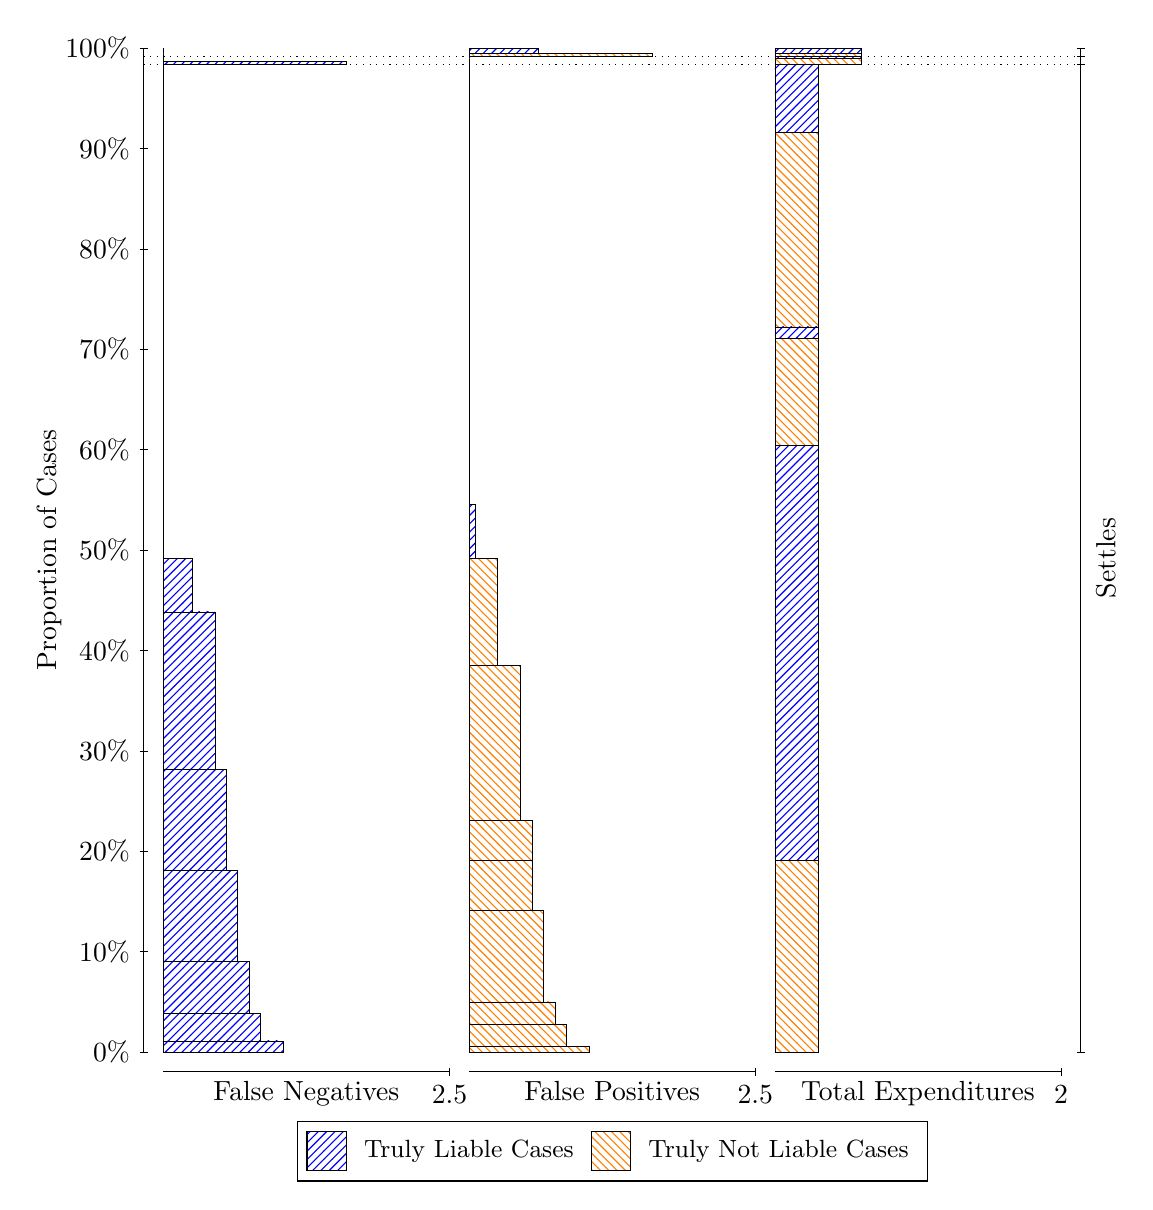
\begin{tikzpicture}
\draw[black, very thin] (1.5,1.75) -- (1.5,14.5);
\node[rotate=90, text=black, anchor=center] at (0.3, 8.125) {Proportion of Cases};
\draw[black, very thin] (1.45,1.75) -- (1.55,1.75);
\node[text=black, anchor=east] at (1.45, 1.75) {0\%};
\draw[black, very thin] (1.45,3.025) -- (1.55,3.025);
\node[text=black, anchor=east] at (1.45, 3.025) {10\%};
\draw[black, very thin] (1.45,4.3) -- (1.55,4.3);
\node[text=black, anchor=east] at (1.45, 4.3) {20\%};
\draw[black, very thin] (1.45,5.575) -- (1.55,5.575);
\node[text=black, anchor=east] at (1.45, 5.575) {30\%};
\draw[black, very thin] (1.45,6.85) -- (1.55,6.85);
\node[text=black, anchor=east] at (1.45, 6.85) {40\%};
\draw[black, very thin] (1.45,8.125) -- (1.55,8.125);
\node[text=black, anchor=east] at (1.45, 8.125) {50\%};
\draw[black, very thin] (1.45,9.4) -- (1.55,9.4);
\node[text=black, anchor=east] at (1.45, 9.4) {60\%};
\draw[black, very thin] (1.45,10.675) -- (1.55,10.675);
\node[text=black, anchor=east] at (1.45, 10.675) {70\%};
\draw[black, very thin] (1.45,11.95) -- (1.55,11.95);
\node[text=black, anchor=east] at (1.45, 11.95) {80\%};
\draw[black, very thin] (1.45,13.225) -- (1.55,13.225);
\node[text=black, anchor=east] at (1.45, 13.225) {90\%};
\draw[black, very thin] (1.45,14.5) -- (1.55,14.5);
\node[text=black, anchor=east] at (1.45, 14.5) {100\%};

\draw[black, very thin] (13.4,1.75) -- (13.4,14.5);
\draw[black, very thin] (13.35,1.75) -- (13.45,1.75);
\node[anchor=west] at (13.35, 1.75) {};
\draw[black, very thin] (13.35,14.296) -- (13.45,14.296);
\node[anchor=west] at (13.35, 14.296) {};
\draw[black, very thin] (13.35,14.398) -- (13.45,14.398);
\node[anchor=west] at (13.35, 14.398) {};
\draw[black, very thin] (13.35,14.5) -- (13.45,14.5);
\node[anchor=west] at (13.35, 14.5) {};

\draw[black, very thin, pattern color=blue, pattern=north east lines] (1.75,1.75) rectangle (3.276,1.8913);
\draw[black, very thin, pattern color=blue, pattern=north east lines] (1.75,1.8913) rectangle (2.9853,2.2441);
\draw[black, very thin, pattern color=blue, pattern=north east lines] (1.75,2.2441) rectangle (2.84,2.8965);
\draw[black, very thin, pattern color=blue, pattern=north east lines] (1.75,2.8965) rectangle (2.6947,4.0564);
\draw[black, very thin, pattern color=blue, pattern=north east lines] (1.75,4.0564) rectangle (2.5493,5.3342);
\draw[black, very thin, pattern color=blue, pattern=north east lines] (1.75,5.3342) rectangle (2.404,7.3397);
\draw[black, very thin, pattern color=blue, pattern=north east lines] (1.75,7.3397) rectangle (2.1133,8.023);
\draw[black, very thin, pattern color=orange, pattern=north west lines] (1.75,8.023) rectangle (1.75,14.296);
\draw[black, very thin, pattern color=blue, pattern=north east lines] (1.75,14.296) rectangle (4.0753,14.33);
\draw[black, very thin, pattern color=orange, pattern=north west lines] (1.75,14.33) rectangle (1.75,14.398);
\draw[black, very thin, pattern color=orange, pattern=north west lines] (1.75,14.398) rectangle (1.75,14.432);
\draw[black, very thin, pattern color=blue, pattern=north east lines] (1.75,14.432) rectangle (1.75,14.5);
\draw[black, very thin, pattern color=orange, pattern=north west lines] (5.6333,1.75) rectangle (7.1593,1.8206);
\draw[black, very thin, pattern color=orange, pattern=north west lines] (5.6333,1.8206) rectangle (6.8687,2.103);
\draw[black, very thin, pattern color=orange, pattern=north west lines] (5.6333,2.103) rectangle (6.7233,2.3852);
\draw[black, very thin, pattern color=orange, pattern=north west lines] (5.6333,2.3852) rectangle (6.578,3.5451);
\draw[black, very thin, pattern color=orange, pattern=north west lines] (5.6333,3.5451) rectangle (6.4327,4.184);
\draw[black, very thin, pattern color=orange, pattern=north west lines] (5.6333,4.184) rectangle (6.4327,4.6954);
\draw[black, very thin, pattern color=orange, pattern=north west lines] (5.6333,4.6954) rectangle (6.2873,6.6565);
\draw[black, very thin, pattern color=orange, pattern=north west lines] (5.6333,6.6565) rectangle (5.9967,8.0231);
\draw[black, very thin, pattern color=blue, pattern=north east lines] (5.6333,8.0231) rectangle (5.706,8.7064);
\draw[black, very thin, pattern color=blue, pattern=north east lines] (5.6333,8.7064) rectangle (5.6333,14.296);
\draw[black, very thin, pattern color=orange, pattern=north west lines] (5.6333,14.296) rectangle (5.6333,14.365);
\draw[black, very thin, pattern color=blue, pattern=north east lines] (5.6333,14.365) rectangle (5.6333,14.398);
\draw[black, very thin, pattern color=orange, pattern=north west lines] (5.6333,14.398) rectangle (7.9587,14.432);
\draw[black, very thin, pattern color=blue, pattern=north east lines] (5.6333,14.432) rectangle (6.5053,14.5);
\draw[black, very thin, pattern color=orange, pattern=north west lines] (9.5167,1.75) rectangle (10.062,4.184);
\draw[black, very thin, pattern color=blue, pattern=north east lines] (9.5167,4.184) rectangle (10.062,9.4516);
\draw[black, very thin, pattern color=orange, pattern=north west lines] (9.5167,9.4516) rectangle (10.062,10.818);
\draw[black, very thin, pattern color=blue, pattern=north east lines] (9.5167,10.818) rectangle (10.062,10.959);
\draw[black, very thin, pattern color=orange, pattern=north west lines] (9.5167,10.959) rectangle (10.062,13.432);
\draw[black, very thin, pattern color=blue, pattern=north east lines] (9.5167,13.432) rectangle (10.062,14.296);
\draw[black, very thin, pattern color=orange, pattern=north west lines] (9.5167,14.296) rectangle (10.607,14.365);
\draw[black, very thin, pattern color=blue, pattern=north east lines] (9.5167,14.365) rectangle (10.607,14.398);
\draw[black, very thin, pattern color=orange, pattern=north west lines] (9.5167,14.398) rectangle (10.607,14.432);
\draw[black, very thin, pattern color=blue, pattern=north east lines] (9.5167,14.432) rectangle (10.607,14.5);
\draw[black, dotted] (1.5,14.296) -- (13.4,14.296);
\draw[black, dotted] (1.5,14.398) -- (13.4,14.398);
\draw[black, very thin] (1.75,1.5) -- (5.3833,1.5);
\node[text=black, anchor=north] at (3.5667, 1.5) {False Negatives};
\draw[black, very thin] (5.3833,1.45) -- (5.3833,1.55);
\node[text=black, anchor=north] at (5.3833, 1.45) {2.5};

\draw[black, very thin] (5.6333,1.5) -- (9.2667,1.5);
\node[text=black, anchor=north] at (7.45, 1.5) {False Positives};
\draw[black, very thin] (9.2667,1.45) -- (9.2667,1.55);
\node[text=black, anchor=north] at (9.2667, 1.45) {2.5};

\draw[black, very thin] (9.5167,1.5) -- (13.15,1.5);
\node[text=black, anchor=north] at (11.333, 1.5) {Total Expenditures};
\draw[black, very thin] (13.15,1.45) -- (13.15,1.55);
\node[text=black, anchor=north] at (13.15, 1.45) {2};

\node[text=black, centered, rotate=90] at (13.72, 8.0231) {Settles};



\draw (7.449999999999999,1.5) node[draw=none] (baseCoordinate) {};
\begin{scope}[align=center]
        \matrix[scale=0.5, draw=black, below=0.5cm of baseCoordinate, nodes={draw}, column sep=0.1cm]{
            \node[rectangle, draw, minimum width=0.5cm, minimum height=0.5cm, pattern color=blue, pattern=north east lines] {}; &
            \node[draw=none, font=\small, text=black] (B) {Truly Liable Cases}; &
            \node[rectangle, draw, minimum width=0.5cm, minimum height=0.5cm, pattern color=orange, pattern=north west lines] {}; &
            \node[draw=none, font=\small, text=black] (B) {Truly Not Liable Cases}; \\
            };
\end{scope}

\end{tikzpicture}
\end{document}